\chapter{Introduction}


\section{Genesis}
    % what is the problem
    Large-scale installations like particle accelerator facilities, metrological laboratories, radar arrays, power grids and many others require monitoring of signals in devices that could be located kilometres away from each other. When the distances are in the range of kilometres the synchronous acquisition of distributed data, presented in Fig. \ref{fig:problem_description}, becomes an issue.
    \begin{figure}
    	\centerline{\includegraphics[width=\textwidth]{figures/problem_description.pdf}}
    	\caption{Demonstration of the synchronous acquisition of distributed data}
    	\label{fig:problem_description}
    \end{figure}
    
    %What is synchronous data acquisition
    Synchronous data acquisition means acquiring data that corresponds to the same moment in time. In a small scale, the difference in time when the data from various sources is acquired depends on the hardware design and the lengths of the cables used to provide the signal to the digitisers. These issues have already been solved in many designs. In large scale, acquisition of the data from various sources at exactly the same time is not straightforward.
    % what are the solutions
    There have been various approaches to solve the problem: 
    \begin{itemize}
        \item The Open Analogue Signal Information System (OASIS) \cite{OASIS}, is currently used at The European Organization for Nuclear Research (CERN) for monitoring the signals in various accelerators. It uses coaxial cables to distribute the trigger signals to all devices. Since all devices receive the same trigger, all signals are acquired at the predefined time.
        \item The LHC Instability Trigger Distribution project (LIST) \cite{LIST_instability_diagnostics}, used at CERN for monitoring the instabilities in the Large Hadron Collider (LHC), uses the White Rabbit (WR) \cite{wr_master} network to distribute the timestamped events and to trigger one device with another with a deterministic delay between the acquisitions. The WR is a deterministic network based on the Synchronous Ethernet and Precision Time Protocol (PTP) \cite{ptp}, which provides subnanosecond synchronisation between the nodes\cite{wr_master}. The WR is described in more detail in section \ref{section:WR}.
        \item The LAN eXtensions for Instrumentation (LXI) \cite{specification:LXI} is a specification that standardises the way various laboratory devices communicate with each other. It introduced various rules for standardising the way the events in devices are timestamped and how the timestamps are distributed.
    \end{itemize}
    All of the approaches, described in more detail in chapter \ref{chapter:existing_solutions}, are very different from each other, yet they have one common goal --- to obtain synchronised data from various devices located far away from each other. 
    
    % what are the solved issues
    Each of the above-mentioned systems has solved some of the following issues relating to synchronous data acquisition in distributed systems:
    \begin{itemize}
        \item a good precision of the synchronisation
        \item scalability
        \item ease of deployment
        \item ease of use
        \item standardisation of the protocol
        \item user-friendly interface
    \end{itemize}
    However, none of them has combined all of the solutions.

    % The reason of DO
    The necessity of providing a system allowing to display the data acquired over large distances, which solves all of the mentioned issues, was the main reason for creating the Distributed Oscilloscope (DO). Having in mind the limitations of the existing solutions, the DO was designed after a deep study of the occurred issues. It uses WR and LXI based White Rabbit Trigger Distribution (WRTD). WRTD's goal is to allow the distribution of the timestamps, which represent the time of various events, between the nodes of the system. It is described in more detail in section \ref{section:WRTD}. Because of the use of the WR network, as well as basing its Application Programming Interface (API) on the LXI, WRTD provides sub-nanosecond synchronisation as well as a standard way of interfacing the devices. In order to ease the deployment of the system, DO uses boards with the Peripheral Component Interconnect Express (PCIe) connectors, so that specialised crates are not necessary to install it. It is written in Python, which is easy to read, understand and modify even for non-programmers. The data transport is optimised so that transmission of large amounts of data does not become an issue. The DO does not require a complex infrastructure, which makes it more scalable. It provides a Graphical User Interface (GUI) designed to be as similar as possible to the standard oscilloscope in order to make it easy to use for every electronics engineer. The DO is not meant to be an operational system, but should serve as a demonstrator of such a system.

\section{Goal} \label{section:goal}
    % the goal
    The goal of the project is to combine the experience gathered from the existing solutions with the use of the available technologies to provide a system allowing to monitor the signals from various devices located far away from each other. The signals should be synchronised by triggering the devices at the time specified by the timestamps. It should provide the functionality of triggering one device based on the event from the other device.

% Assumptions
\section{Assumptions and requirements} \label{section:assumptions_and_requirements}
    Taking into account the limitations caused by the available hardware, the project was created with the following assumptions:
    \begin{itemize}
        \item Since only two digitiser boards (see section \ref{section:fmc_adc}) were available, the actual measurements should be carried out on them. Connecting more devices should be possible.
        \item The possibility of synchronising the devices over distances in the range of kilometres (the fibre used during the development has a length of 2.5~km).
        \item Since the used digitiser boards have the timestamping clock not locked to the sampling clock, the minimum precision of synchronisation should be no worse than $\pm (T_s + 1~ns)$, where $T_s$ is a sampling clock period.
        \item It should be easy to distribute to the users. The requirement of CERN is that it is written in Python.
        \item It should provide a user-friendly interface. The requirement of CERN is that the GUI is written with the use of Qt (see section \ref{section:general_architecture}).
        \item The final application should be easily extendable. An example of a tool that could use the synchronisation features of the DO is Phase Measurement Unit (PMU). It is a tool used for measuring the phase difference between the signals.
        \item The digitisers are installed in one or more computers with PCIe slots.
        \item The drivers and all the required C libraries are provided by CERN.
        \item The application is the first use of the WRTD. The work should provide feedback and help to resolve the existing issues before the first release.
        \item The user should be able to control the behaviour of the necessary configuration of the devices, but the synchronisation details should be hidden.
    \end{itemize}

The current chapter describes the problem of the synchronous data acquisition, already existing solutions and a brief description of the DO. In order to clarify the reason for creating the DO, the already mentioned existing solutions are described in more detail in chapter 2.



%\textcolor{blue}{Write it after finishing the rest of the chapters}
%\textcolor{blue}{Describe the problem of the acquisition of the data of the distributed system}
%\textcolor{blue}{Write shortly about LXI, OASIS, the system used in the LHC}
%\textcolor{blue}{Describe the existing solutions}
%\textcolor{blue}{Write shortly about the distributed oscilloscope}

% \section{Genesis}
% Problem of acquisition of the data in large distributed systems.
% Describe shortly the existing solutions.
% Expose the problems of the existing solutions.

% \section{Goal}
% Describe how to make the existing solutions better. 
% How it can be achieved with the use of the new technologies. --- WR, WRTD.
% Describe here the functionality of the DO that You have obtained. More or less the thing that Javier and Dimitris told You at the begining.

% \section{Assumptions}
% minimum 2 boards
% minimum distance of 2.5 km
% available precision depending on the board and locking of the clock
% easy to distribute
% scalable
% working with any number of devices --- I am limited with the available boards
% possible to expand into something more, eg. PMU

% existing solution:                                                             
%     - apples and oranges                                                        
                                                                                
% introduction:                                                                   
%     - genesis                                                                   
%         - description of the problem                                            
%         - briefly touch the existing solutions                                  
%         - new technology WR, WRTD                                               
%     - set the goals                                                             
%         - precision                                                             
%         - user friendlyness - LIST is not user friendly, it exposes the low level mechanisms                                             
%         - scalability                                                           
%         - first use of the ADCs triggering and being triggered in the           
%           WR network. Before there was only with external ADCs                 
%         - long distances                                                        
%     - assumptions and requirements given by CERN                                
%         - thinks given to use, FMC ADC 100M, 2-5 ADC boards, FEC and            
%           desktop, drivers, libraries, WRTD, synchronization within             
%           2 samples of the ADC, 10 km, python, QT, 